%% One-page panel: rho's native observation logic forces two bounds.
\documentclass[11pt]{article}
\usepackage[margin=2.2cm]{geometry}
\usepackage{amsmath,amssymb}
\usepackage{tikz}
\usetikzlibrary{arrows.meta,positioning}
\usepackage{booktabs}
\newcommand{\code}[1]{\texttt{#1}}
\pagestyle{empty}

\begin{document}

\begin{center}
{\Large\bfseries Rho's native observation logic forces two bounds}\\[2pt]
{\small kernel-checked in Lean 4; axioms: \code{propext},
\code{Classical.choice}, \code{Quot.sound}}
\end{center}

\vspace{4pt}
\begin{center}
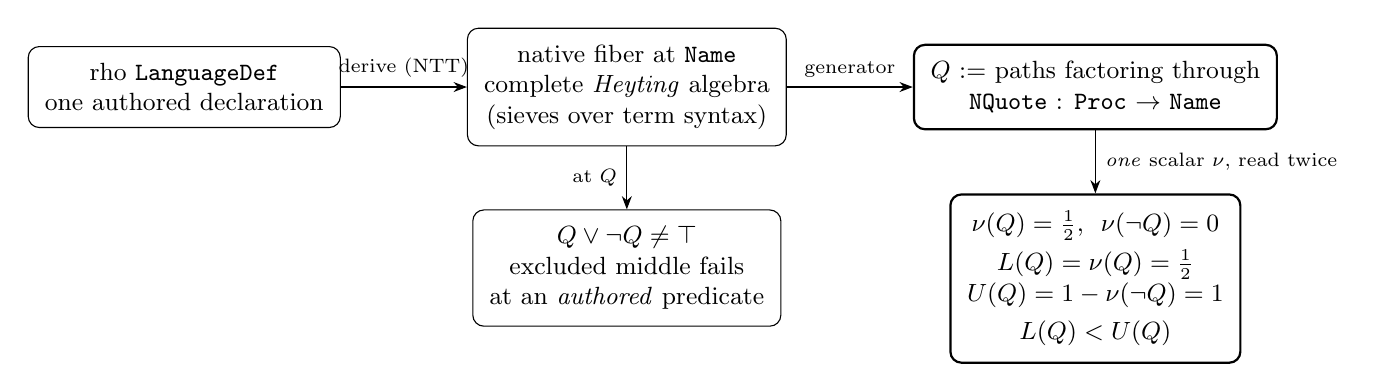
\begin{tikzpicture}[node distance=6mm and 16mm,
  box/.style={draw, rounded corners, align=center, inner sep=6pt,
    font=\small},
  hot/.style={draw, rounded corners, align=center, inner sep=6pt,
    font=\small, thick}]
\node[box] (ld) {rho \code{LanguageDef}\\one authored declaration};
\node[box, right=of ld] (fib) {native fiber at \code{Name}\\complete
  \emph{Heyting} algebra\\(sieves over term syntax)};
\node[hot, right=of fib] (q) {$Q$ := paths factoring through\\
  \code{NQuote} : \code{Proc} $\to$ \code{Name}};
\node[box, below=8mm of fib] (em) {$Q \lor \lnot Q \ne \top$\\
  excluded middle fails\\at an \emph{authored} predicate};
\node[hot, below=8mm of q] (nums)
  {$\nu(Q)=\tfrac12$,\ \ $\nu(\lnot Q)=0$\\[3pt]
   $L(Q)=\nu(Q)=\tfrac12$\\
   $U(Q)=1-\nu(\lnot Q)=1$\\[3pt]
   $L(Q) < U(Q)$};
\draw[-{Stealth}] (ld) -- (fib)
  node[midway,above,font=\scriptsize]{derive (NTT)};
\draw[-{Stealth}] (fib) -- (q)
  node[midway,above,font=\scriptsize]{generator};
\draw[-{Stealth}] (fib) -- (em)
  node[midway,left,font=\scriptsize]{at $Q$};
\draw[-{Stealth}] (q) -- (nums)
  node[midway,right,font=\scriptsize]{\emph{one} scalar $\nu$, read
    twice};
\end{tikzpicture}
\end{center}

\vspace{2pt}
\noindent\textbf{One ruler, two readings.}  The valuation $\nu$ is a
single scalar map on the fiber.  Read directly it reports
\emph{support}: $L(a)=\nu(a)$.  Read through the lattice's own negation
it reports \emph{non-refutation}: $U(a)=1-\nu(\lnot a)$.  Boolean
excluded middle would force $L=U$.  Rho's quote-generated predicate
keeps them apart --- so no single point value can play both semantic
roles, and a complete plausibility report about $Q$ is the pair
$(L,U)=(\tfrac12,\,1)$.

\vspace{6pt}
\noindent\textbf{Why the gap appears.}  \code{NQuote} lies in $Q$; the
identity on \code{Name} does not; naturality forbids the complement from
containing the identity while excluding its restriction along
\code{NQuote}.  The failure of excluded middle is the constructor
geometry of quoting, nothing imported.

\vspace{6pt}
\begin{center}
\small
\begin{tabular}{@{}ll@{}}
\toprule
Lean declaration & establishes \\
\midrule
\code{rhoQuotePredicate\_excludedMiddle\_ne\_top} &
  $Q \lor \lnot Q \ne \top$ \\
\code{rhoNameNativeFiber\_not\_boolean} &
  the fiber is non-Boolean \\
\code{rhoCalc\_nativeType\_requires\_distinct\_probability\_bounds} &
  $L(Q)=\tfrac12 < 1 = U(Q)$ \\
\bottomrule
\end{tabular}
\end{center}

\vspace{6pt}
\noindent\textbf{Scope, stated exactly.}  The witness is structural ---
constructor/presheaf geometry, not \textsc{comm} nondeterminism; the
operational $\Diamond/\Box$ connection is future work.  The theorem
concerns two independently meaningful readouts, not encoding
cardinality.  Knuth--Skilling fidelity is used in its published one-way
form, and their quantum pair postulate is not invoked.  \emph{Which}
two-component algebra to adopt (evidence pairs, amplitude--phase, \dots)
remains a genuine choice with genuinely different capabilities; whether
a \emph{point} value suffices for rho's native logic does not.

\end{document}
